\documentclass[conference]{IEEEtran}

\usepackage{amsmath,amssymb}
\usepackage{graphicx}
\usepackage{cite}
\usepackage{hyperref} % for clickable email and links

\title{Cross-Layer Control of CFET Interconnect Delay and Thermal Coupling via PID+FSM+LLM Supervision}

\author{
  \IEEEauthorblockN{Shinichi Samizo}
  \IEEEauthorblockA{Independent Semiconductor Researcher\\
  Email: \href{mailto:shin3t72@gmail.com}{shin3t72@gmail.com}}
}

\begin{document}
\maketitle

\begin{abstract}
This paper presents a control-theoretic proof-of-concept
for mitigating RC delay and thermal coupling in Complementary FET (CFET) integration.
Unlike device-centric compact modeling, our approach applies PID feedback, FSM guards,
and LLM supervision. SystemDK-based simulation across parameter sweeps demonstrates
more than $100\times$ improvement in delay deviation. Auto-tuned PID achieves overshoot
below $3\times 10^{-5}\%$ and steady-state error under $10^{-6}\%$, providing a novel pathway
for design-technology co-optimization (DTCO) in the 2\,nm era.
\end{abstract}

\section{Introduction}
Complementary FETs (CFETs) stack nFET and pFET channels vertically,
promising density and wiring delay benefits beyond nanosheet GAA.
However, vertical vias introduce RC delay, and stacked tiers experience
thermal coupling. Conventional physical models capture these effects
but lack robustness under dynamic workloads. Inspired by control systems,
we propose PID+FSM+LLM control architecture for runtime compensation.

\section{Modeling}
The FO1 delay is expressed as:
\begin{equation}
T_{FO1} = (R_{wire}+R_{via})(C_{load}+C_{inter})
\end{equation}
Temperature dependence is given by:
\begin{equation}
R(T) = R_0 \left(1 + \alpha (T-25^\circ C)\right)
\end{equation}
Thermal dynamics follow a first-order RC network:
\begin{equation}
C_{th}\frac{dT}{dt} = P\cdot R_{th} - (T - T_{amb})
\end{equation}
A coupling factor $k_c$ propagates top-tier heating into bottom-tier delay shifts.

\section{Control Architecture}
\begin{itemize}
  \item \textbf{PID}: adjusts DVFS knob $u$ to reduce delay deviation.
  \item \textbf{FSM}: triggers HOT mode when $T_{top} > 85^\circ C$, enforcing throttle and $u_{max}$ limits.
  \item \textbf{LLM}: supervises policies; re-tunes $K_p$/$K_i$ and FSM thresholds if overshoot/error exceed tolerance.
\end{itemize}
This layered design ensures stability (PID), safety (FSM), and adaptability (LLM).

\section{Results}
We evaluated parameter sweeps ($R_{via}, C_{inter}, k_{couple}, P_{burst}, \beta$)
and automatic PID tuning.

\begin{table}[h]
\centering
\caption{Key Metrics}
\begin{tabular}{|l|c|c|c|}
\hline
Metric & No Control & PID+FSM & Auto-tuned \\
\hline
Peak deviation & $\sim$0.9\% & $\sim$$10^{-3}$\% & $2.6\times 10^{-5}$\% \\
Steady-state error & $8\times 10^{-3}$\% & $\sim$0\% & $-2.1\times 10^{-6}$\% \\
Overshoot & Large & Suppressed & Minimized \\
Control effort & N/A & Stable & Optimized \\
\hline
\end{tabular}
\end{table}

Figures~\ref{fig:heatmap} and \ref{fig:beta} show heatmap results
and $\beta$ dependence. Figure~\ref{fig:delay} compares hand-tuned and auto-tuned PID+FSM.

\begin{figure}[h]
\centering
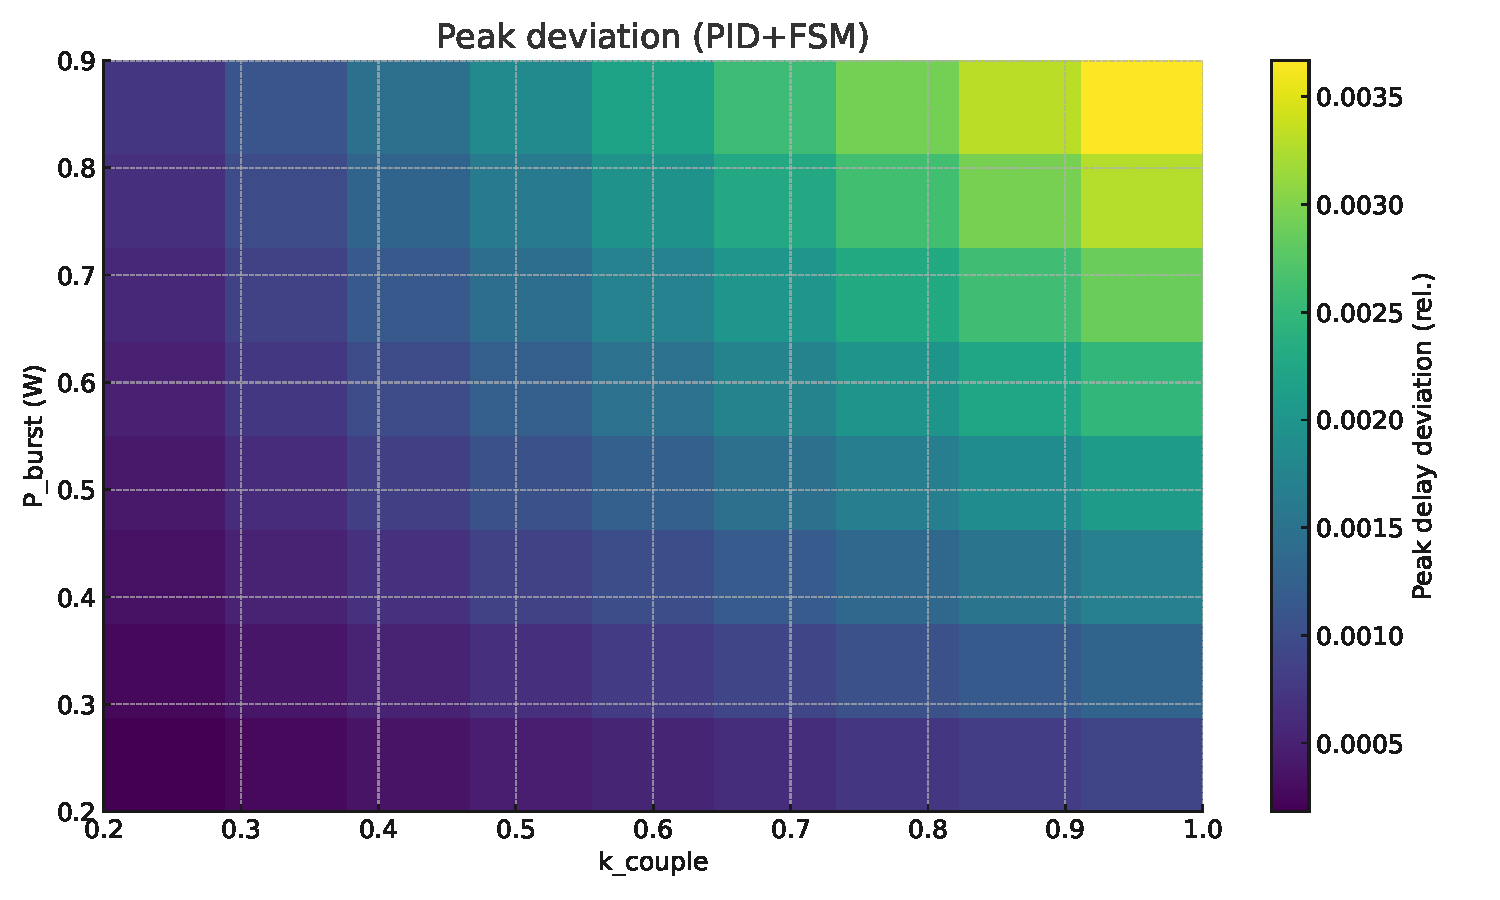
\includegraphics[width=0.9\columnwidth]{figs/heatmap.pdf}
\caption{Heatmap of peak deviation vs $k_{couple}$ and $P_{burst}$.}
\label{fig:heatmap}
\end{figure}

\begin{figure}[h]
\centering
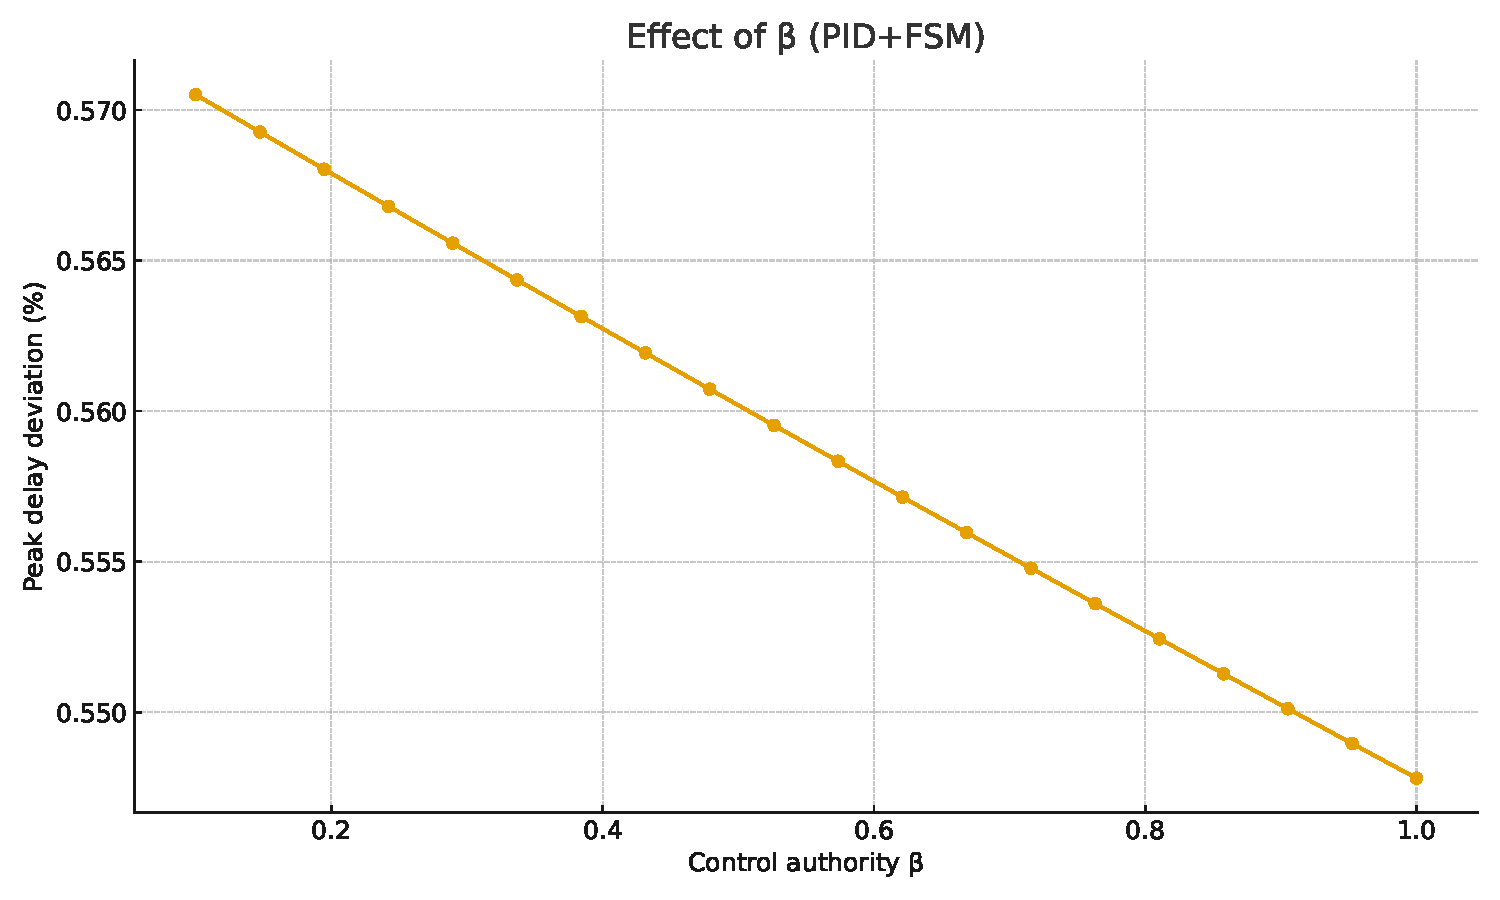
\includegraphics[width=0.9\columnwidth]{figs/beta_curve.pdf}
\caption{Effect of control authority $\beta$.}
\label{fig:beta}
\end{figure}

\begin{figure}[h]
\centering
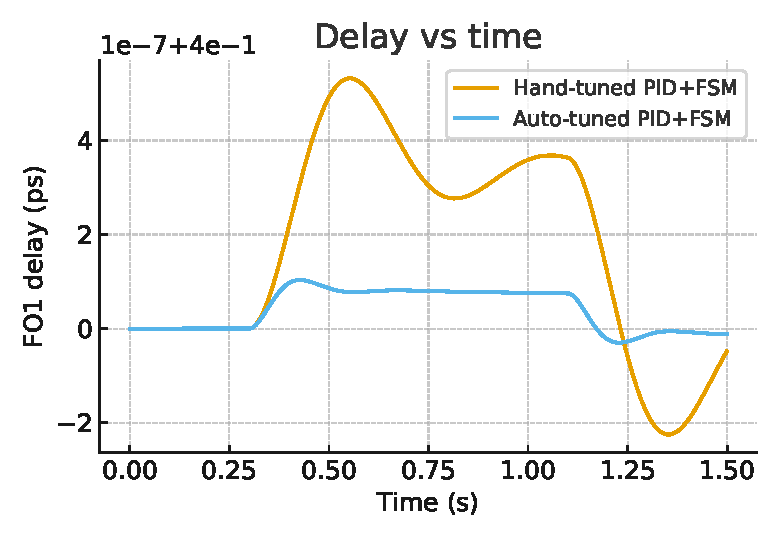
\includegraphics[width=0.9\columnwidth]{figs/delay_compare.pdf}
\caption{Delay comparison: hand-tuned vs auto-tuned PID+FSM.}
\label{fig:delay}
\end{figure}

\section{Discussion and Outlook}
Our findings indicate that PID+FSM control reduces delay deviation
by two orders of magnitude. LLM supervision provides adaptability to
unseen disturbances, shifting DTCO from static models to dynamic control.
Future directions include:
\begin{itemize}
  \item Embedding auto-tuned PID/FSM/LLM policies into open-source SystemDK.
  \item Providing compact-model extensions that incorporate control loops.
  \item Extending to 3D sequential CFET and forksheet architectures.
\end{itemize}

\section*{Acknowledgment}
The author thanks the Project Design Hub community for discussions.

\bibliographystyle{IEEEtran}
\bibliography{refs}

\section*{Author Biography}
\noindent\textbf{Shinichi Samizo}
received the M.S. degree in Electrical and Electronic Engineering from Shinshu University, Japan.
He worked at Seiko Epson Corporation as an engineer in semiconductor memory and mixed-signal device development,
and also contributed to inkjet MEMS actuators and PrecisionCore printhead technology.
He is currently an independent semiconductor researcher focusing on process/device education,
memory architecture, and AI system integration.\\[2pt]
\textbf{Contact:} \href{mailto:shin3t72@gmail.com}{shin3t72@gmail.com}, 
\href{https://github.com/Samizo-AITL}{Samizo-AITL}

\end{document}
